\documentclass[a4paper]{article}
\usepackage[letterpaper, margin=1in]{geometry} % page format
\usepackage{listings,graphicx,amsmath, amssymb, amsfonts, amsthm,tikz,hyperref,fullpage,setspace,enumerate,mathtools,arydshln} 

\title{Homework 2}
\author{Helen Ngo}
\date{\today}

\begin{document}
\lstset{language=Python}

\maketitle

\begin {description}

\item[Problem 2.1] In Equation (2.1), set $\delta = 0.03$ and let 
\[\epsilon(M, N, \delta) = \sqrt{\frac{1}{2N}\ln\frac{2M}{\delta}}.\]

\begin{enumerate}[(a)]
\item For $M=1$, how many examples do we need to make $\epsilon \leq 0.05$?
\item For $M=100$, how many examples do we need to make $\epsilon \leq 0.05$?
\item For $M=10,000$, how many examples do we need to make $\epsilon \leq 0.05$?
\end{enumerate}

\smallskip

\textbf{Solution:}
\begin{doublespace}
\begin{enumerate}[(a)]

\item Let 
\begin{equation}
 	\begin{aligned}
	\label{eq1}
		\epsilon(M, N, \delta) = \sqrt{\frac{1}{2N}\ln\frac{2M}{\delta}},
 	\end{aligned}
\end{equation}

where $\epsilon \leq 0.05$, $M = 1$ and $\delta = 0.03$. Then
\begin{align*}
0.05 &\geq \epsilon(M, N, \delta) = \sqrt{\frac{1}{2N}\ln\frac{2}{0.03}} \\
0.0025 &\geq \frac{1}{2N}\ln\frac{2}{0.03} \\
0.0025\left( \ln\frac{2}{0.03} \right)^{-1} &\geq \frac{1}{2N} \\
400 \ln\frac{2}{0.03} &\leq 2N \\
200 \ln\frac{2}{0.03} &\leq N \\
~839.941 &\leq N \\
N &\geq 840.
\end{align*}
We need at least $N \geq 840$ examples to make $\epsilon \leq 0.05$ for $M=1$.

\item Substituting $\epsilon \leq 0.05$, $M = 100$ and $\delta = 0.03$ into equation \eqref{eq1}, we can solve for $N$,
\begin{align*}
0.05 &\geq \sqrt{\frac{1}{2N}\ln\frac{200}{0.03}} \\
0.0025 &\geq \frac{1}{2N}\ln\frac{200}{0.03} \\
0.0025\left( \ln\frac{200}{0.03} \right)^{-1} &\geq \frac{1}{2N} \\
400 \ln\frac{200}{0.03} &\leq 2N \\
200 \ln\frac{200}{0.03} &\leq N \\
~1761.975 &\leq N \\
N &\geq 1762.
\end{align*}
We need at least $N \geq 1762$ examples to make $\epsilon \leq 0.05$ for $M=100$.

\item Notice that between $M = 1$ and $M = 100$, only one number changes in the result before the answer. Thus, for $M = 10,000$,
\[N \geq 200 \ln\frac{20,000}{0.03} \approx 2682.009 = 2683.\]
We need at least $N \geq 2683$ examples to make $\epsilon \leq 0.05$ for $M=10,000$.

\end{enumerate}
\end{doublespace}

\newpage

\item[Problem 2.11] Suppose $m_H(N) = N + 1$, so $d_{vc} = 1$. You have $100$ training examples. Use the generalization bound to give a bound for $E_{\mathrm{out}}$ with confidence $90\%$. Repeat for $N = 10,000$.

\smallskip

\textbf{Solution:}
\begin{doublespace}
The generalization bound states, "For any tolerance $\delta > 0$
\begin{equation}
 	\begin{aligned}
	\label{eq2}
		E_{\mathrm{out}} \leq E_{\mathrm{in}} + \sqrt{\frac{8}{N} \ln \frac{4m_H(2N)}{8}}
 	\end{aligned}
\end{equation}
with probability $\geq 1 - \delta$."
Substitute $N = 100$ into equation \eqref{eq2},
\begin{align*}
E_{\mathrm{out}} &\leq E_{\mathrm{in}} + \sqrt{\frac{8}{N} \ln \frac{4m_H(2N)}{8}} \\
&= E_{\mathrm{in}} + \sqrt{\frac{8}{100} \ln \frac{4(2\times100+1)}{8}} \\
&\approx E_{\mathrm{in}} + \sqrt{0.3688} \\
&\approx E_{\mathrm{in}} + 0.6073.
\end{align*}
The bound for $E_{\mathrm{out}} \leq E_{\mathrm{in}} + 0.6073$. Similarly, for $N = 10,000$, the bound is
\[E_{\mathrm{out}} \leq E_{\mathrm{in}} + \sqrt{\frac{8}{10000} \ln \frac{4(2\times10000+1)}{8}} \approx E_{\mathrm{in}} + 0.0858.\]
\end{doublespace}

\item[Problem 2.12] For an $H$ with $d_{vc} = 10$, what sample size do you need to have a $95\%$ confidence that your generalization error is at most $0.05$?

\smallskip

\textbf{Solution:}
\begin{doublespace}
Using equation (2.13), we need
\[N \geq \frac{8}{0.05^2} \ln \left( \frac{4(2N)^{10}+4}{0.05} \right).\]
Trying an initial guess of $N_0= 1,000$ in the RHS, we get
\[N \geq \frac{8}{0.05^2} \ln \left( \frac{4(2\times1000)^{10}+4}{0.05} \right) \approx 257,251.\] 
Then we try the new value $N = 257,251$ in the righthand side and continue the iterative process until $N_i/N_{i-1} \approx 1$. The iterative process converges to an estimate of $N \approx 451,652$.
\end{doublespace}

\newpage

\item[Problem 3.1] Consider the double semi-circle ``toy" learning task. This task is linearly separable when $sep \geq 0$, and not so for $sep < 0$. Set $rad =10, thk = 5$ and $sep = 5$. Then, generate $2,000$ examples uniformly, which means you will have approximately $1,000$ examples for each class.
\begin{enumerate}[(a)]
\item Run the PLA starting from $\mathbf{v} = \mathbf{0}$ until it converges. Plot the data and the final hypothesis.
\item Repeat part (a) using the linear regression (for classification) to obtain $\mathbf{w}$. Explain your observations.
\end{enumerate}

\smallskip

\textbf{Solution:}
\begin{doublespace}
The python code is attached.
\begin{enumerate}[(a)]
\item Adjusting the Perceptron from Assignment 1, so that the points are generated by the function $make\_semi\_circles$, we can run the PLA as before. The plot below shows the data and the final hypothesis as produced by PLA.

\begin{center}
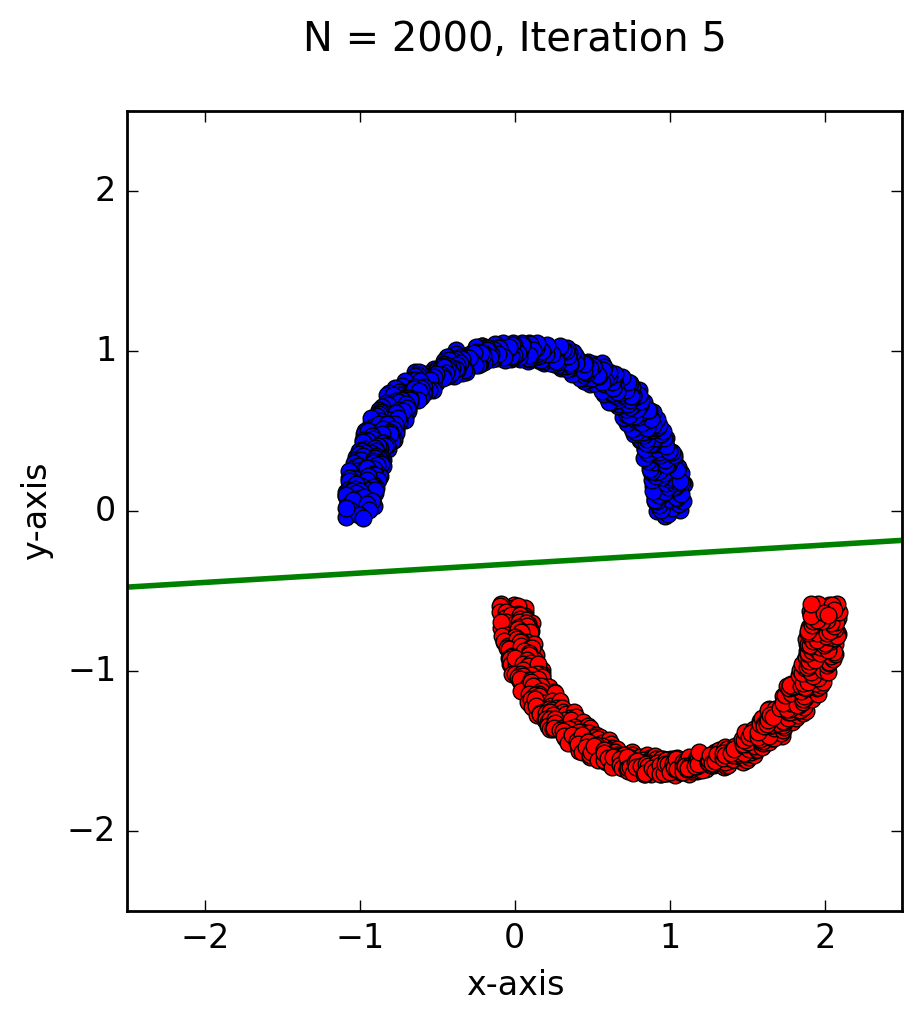
\includegraphics[scale=0.75]{Problem_3_1a.png}
\end{center}

\newpage

\item The $linear\_regression$ function added to the Perceptron code so that using the same point, a linear classification line was produced. The classification line, produced using the same data as part (a), is shown in the plot below.

\begin{center}
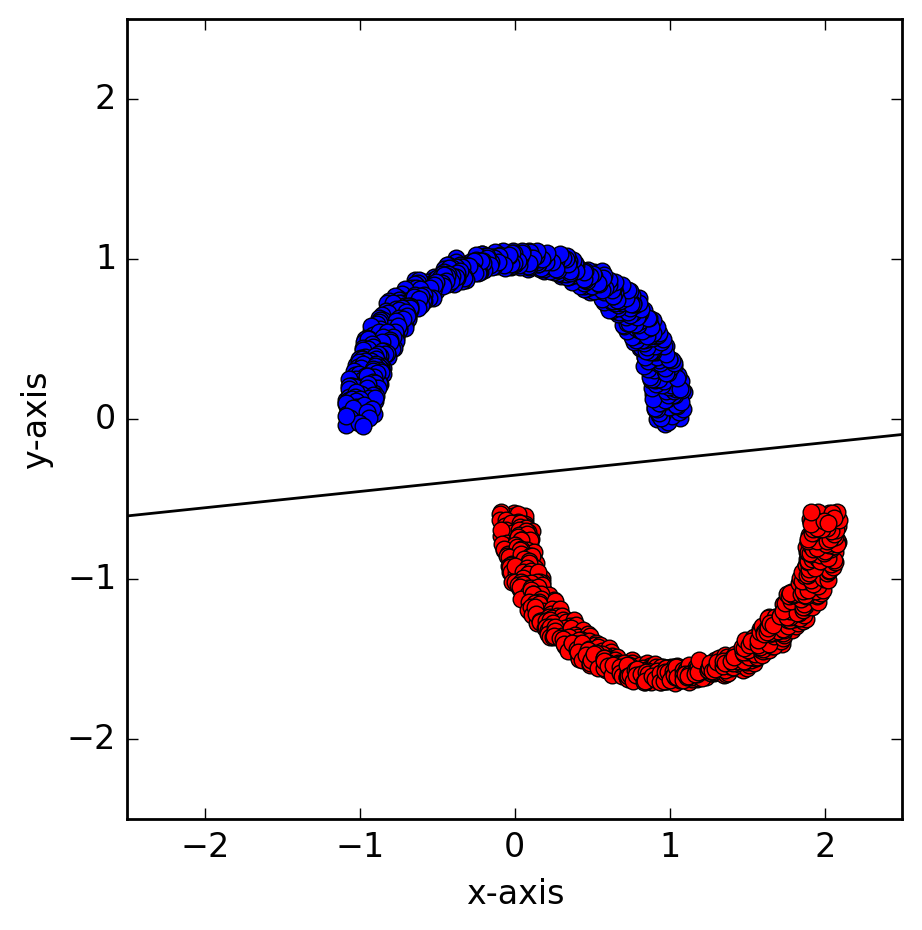
\includegraphics[scale=0.65]{Problem_3_1b.png}
\end{center}

While the separating lines above are similar, linear regression classification will always give us the line with the lowest variance while the PLA just produces a separating line. This can be better observed for another set of data, the linear regression line and perceptron line are shown below for it.

\begin{center}
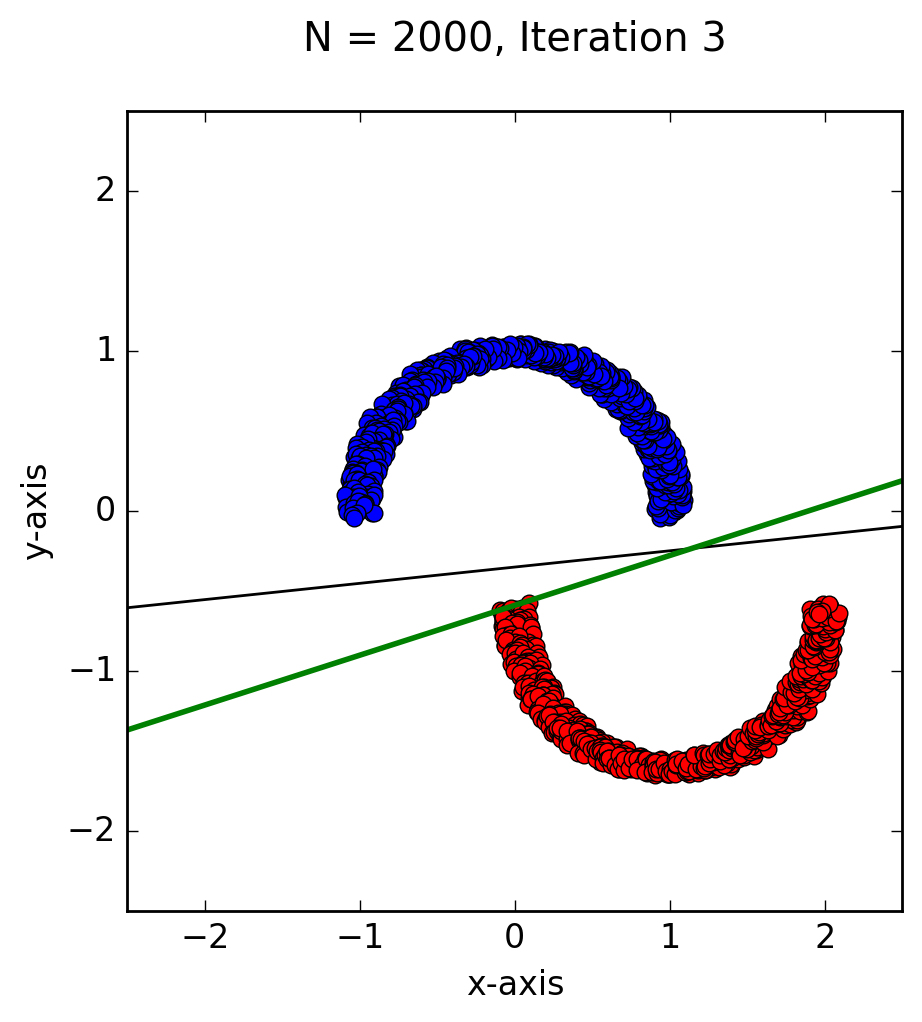
\includegraphics[scale=0.65]{Problem_3_1_c.png}
\end{center}

\end{enumerate}
\end{doublespace}

\item{Problem 3.2} For the double-semi-circle task, vary $sep$ in the range $\{0.2,0.4,...,5\}$.

\smallskip

\textbf{Solution:}
\begin{doublespace}
Despite the varying size of the separation between semi-circles $sep$, the number of iterations that the PLA ran remained relatively constant; no relationship between $sep$ and number of iterations could be determined. In the plot below, the y-axis is the frequency and the x-axis is the $sep$. 

\begin{center}
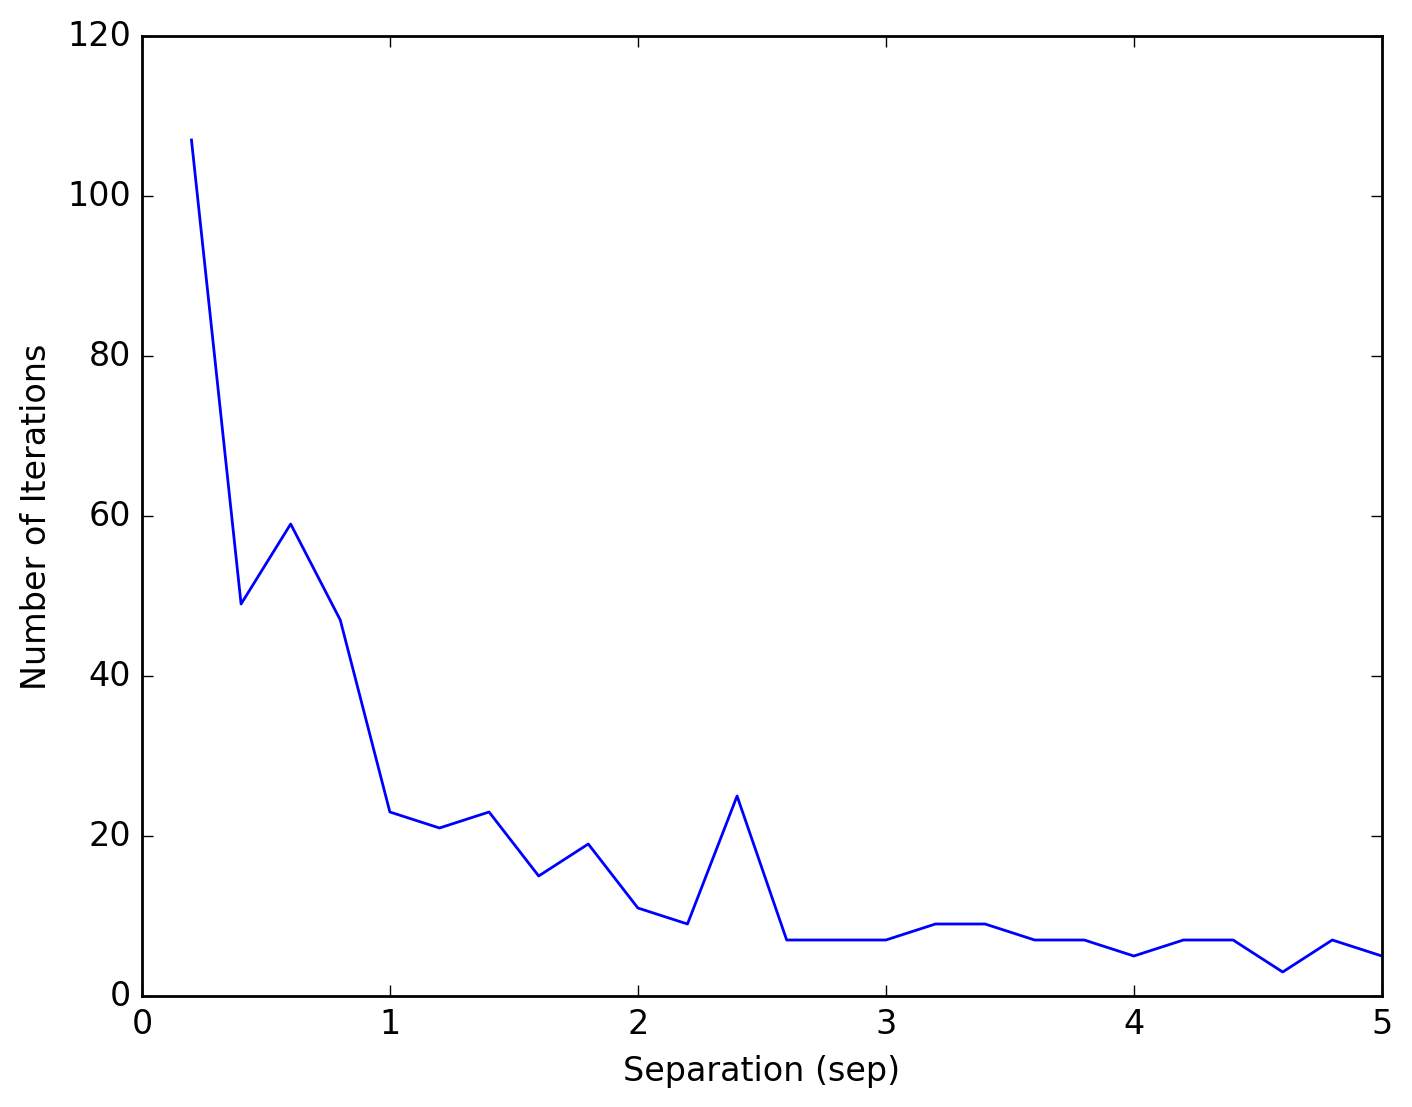
\includegraphics[scale=0.65]{Problem_3_2.png}
\end{center}
\end{doublespace}


\end {description}
\end{document}
